% generated by make_combined.py from stage8_labels_strong_model/stage8.tex; do not edit
\section{Stage 8 --- Are the real-artifact labels right, and does the law hold for a strong model?}\label{sec:stage8}

\stagebox{\textbf{In one sentence.} Checked without a clinician --- against three public expert annotation sets and two
independent automatic labellers --- the dermoscopy labels of Stage~3 put hair on the correct side of the lesion boundary
but mark hair on many images that experts call hair-free, and removing every image an independent source contradicts
\emph{increases} the crossover (\sEightOrigisic{} $\to$ \sEightCleanisic); the thyroid caliper labels agree with two
independent labellers wherever those agree with each other, but the registered cleaning rule removed too many images for
its test to run; the ovary and capsule labels could not yet be checked; and a fine-tuned thyroid model \sEightFTZeroGap{}
AUROC below the published benchmark shows every registered harm of masking, including a sensitivity loss from
\sEightConfErmOPTwo{} to \sEightConfMaskOPTwo{} in the \sEightSubN{} malignant nodules with a caliper on the nodule, a
subgroup now registered before any result.}
\subsection{Where this stage starts}
Stages~1--7 established the location law --- ROI masking removes an out-of-ROI shortcut and keeps, or amplifies, an
in-ROI one --- and showed that it holds across masking implementations, is graded in the real overlap and appears on an
external test set (Stage~7). Two objections remained that the earlier stages could not answer with their own data:
\begin{enumerate}[leftmargin=*]\itemsep1pt
\item \emph{``Nobody checked the real-artifact labels.''} The real traps of Stage~3 rest on automatic labels: published
hair masks \citep{wegley2026artifacts}, a rule-based caliper detector (thyroid, ovary), a contamination probe (capsule)
and lesion masks that are partly U-Net predictions. The audit package of Stage~6 was prepared for a clinician, and no
clinician is available to rate it.
\item \emph{``The thyroid model is weaker than published ones, and the subgroup was chosen after the fact.''} The frozen
probe of Stage~5 reaches a test AUROC of \sEightFrozenAuc{} on the official patient-disjoint split, below the fine-tuned
models of \citet{gong2022acl} (0.773--0.799); the \sEightSubN{} malignant nodules with an in-ROI caliper, in which masking
cost most sensitivity, were defined post hoc.
\end{enumerate}
This stage answers both with one registration (Part A: labels; Part B: a fine-tuned model), committed with three
amendments before any analysis.

\subsection{Questions}
\begin{enumerate}[label=\textbf{Q8\alph*},leftmargin=*]\itemsep1pt
\item How often do independent sources contradict our artifact labels, and do the errors differ by diagnosis?
\item Does the crossover survive on the images that no independent source contradicts?
\item Does a fine-tuned model close to the published benchmark show the harms that masking caused the frozen probe?
\item Does the subgroup harm hold when the subgroup is registered in advance?
\end{enumerate}
\paragraph{Design decisions} \emph{Why a clinician-free check is enough for these claims.} Whether a hair crosses a lesion,
a caliper lies on a nodule or debris lies inside a box is a visual fact, not a diagnosis, and the claims of Stage~3 need
only these facts. Moreover, if trap membership is misclassified independently of the diagnosis, the observed crossover is
attenuated, $C_{\text{obs}}\approx(1-e_A-e_B)\,C_{\text{true}}$: random label errors shrink a crossover and cannot create
one. The checks therefore measure the error rates, test whether they differ by diagnosis, and re-run the traps without the
contradicted images. \emph{Sources.} Public expert annotations where they exist: DermArtifactDB for hair presence
\citep{dermartifactdb}, IMA++ lesion masks \citep{imapp}, the hair masks of \citet{kabirhair} and expert contamination masks
for capsule frames \citep{capsulemasks}. No public caliper annotation exists, so two independent automatic labellers are
used for calipers: BUSClean, an ultrasound annotation detector \citep{busclean}, and MedGemma, a medical vision--language
model \citep{medgemma}, both run locally. \emph{Safeguards} (Amendments~1--2): images on which one of our own labellers was
trained are excluded from every comparison; a source is analysed only if it covers at least 200 of our images; a model
labeller counts only if its $\kappa$ is at least 0.40 on the images on which the two other caliper labels agree; BUSClean
is declared invalid if it fires on more than half of our caliper-free images; neither model labeller is ever shown our
artifact masks. \emph{Rating.} A blinded rating of the audit sample by the author (a non-clinician) is registered (A4);
it has not been done yet and does not enter the results below. \emph{Part B.} The recipe is chosen on validation images
only; the benchmark is the lowest published cross-entropy baseline on the same split (0.773).

\subsection{Methods}
\paragraph{A0 --- sources and coverage} Each source's licence was read from the source itself and recorded before use.
Matching: ISIC by image identifier; capsule frames by perceptual hash (Hamming distance $\le2$, as in Stage~1). IMA++ is
used as a majority mask over its annotators; its masks and anything derived from them at pixel level stay on the GPU
machine (CC BY-NC-ND). The coverage report was committed before any agreement was computed.
\paragraph{A1 --- agreement} Hair: $\kappa$ of our hair-free status ($\le30$ hair pixels) with DermArtifactDB; Dice of our
hair masks with the Kabir masks. Lesion masks: Dice with the IMA++ majority mask, and the trap class recomputed with it
(like for like at 518\,px). Calipers: $\kappa$ of presence with BUSClean and with MedGemma; for location, agreement of
our class with BUSClean's detected positions and with MedGemma's answer to ``is any caliper mark inside the green
contour?'' on the image with only the nodule outline drawn. MedGemma: fixed prompts, greedy decoding, answer parsed as
yes/no. Every agreement is reported for $Y=0$ and $Y=1$ separately.
\paragraph{A2 --- traps on uncontradicted labels} Contradicted images are removed; images without an independent source
are kept. The Stage~3 protocol is re-run unchanged (DINOv2 ViT-B/14 at 518\,px, same matching, seeds and folds, ERM and
mask arms, crossed bootstrap) with the count gate of Stage~7 ($\ge25$ images per matched cell). HA2: crossover $>0$ in
every cohort that passes the gate (Holm).
\paragraph{A3 --- differential error} Error rates of our cells against every informative source by trap and diagnosis;
differential error is flagged if the rates for $Y=1$ and $Y=0$ differ by more than 0.10 with a CI excluding zero, and a
flagged cohort's conclusion then rests on A2. The attenuation correction is reported only for unflagged cohorts.
\paragraph{Part B --- fine-tuned thyroid model} Twelve recipes (ConvNeXt-T, ResNet-50, DINOv2 ViT-B/14 $\times$ two
learning rates $\times$ 8 or 20 epochs; 224\,px, the training procedure of Stage~5) are compared by validation AUROC of
ERM, seed 42. The chosen recipe is then trained on the natural split (5 seeds $\times$ ERM, mask, balanced, mask +
balanced; validation predictions saved for the operating points) and in the thyroid traps (2 environment seeds $\times$ 5
folds = 10 bootstrap clusters). FT0 (descriptive): mean ERM test AUROC $\ge0.773$. FT1: hard-pair AUROC, mask $-$ ERM $<0$.
FT2: sensitivity CI below zero at $\ge3$ of OP2--OP5. FT3: at OP2, sensitivity of the malignant nodules with an in-ROI
caliper, mask $-$ ERM $<0$. FT4: trap crossover $>0$. Holm over FT1--FT4.
\paragraph{E1--E2 --- exploratory} Decided after A1--A3 were known and reported separately: a consensus view in which an
image counts as contradicted only if both caliper labellers place it in the same cell and that cell differs from ours
(E1), and FT3 restricted to the subgroup nodules that both labellers confirm (E2).

\subsection{Experiments}
\begin{table}[H]\centering\scriptsize
\caption{Experiments of this stage. \texttt{docs/PREREGISTRATION\_ROUND6.md} and its three amendments were committed before any analysis of this round; the coverage report (\sEightCommitCoverage), the fine-tune recipe (\sEightCommitRecipe) and the hash of the A4b key (\sEightCommitAfourb) were committed before the steps that use them. Commit times are set by the committing machine and are not independent proof of order.}\label{s8:tab:exp}
\begin{tabular}{p{3.8cm}p{3.4cm}p{2.8cm}p{5.0cm}}\toprule
Experiment & Status & First commit (local time) & Support criterion \\\midrule
A0 sources, licences, coverage & \registered{round 6}; coverage committed before A1 & \texttt{607900c}, 2026-09-28 14:27 & $\ge200$ matched images: analysed; 50--199: descriptive; $<50$: not feasible \\
A1 agreement with independent sources & \registered{round 6} & \texttt{607900c}, 2026-09-28 14:27 & descriptive; a model labeller is used only if $\kappa\ge0.40$ (Amendment 2: validity guard) \\
A2 traps on uncontradicted labels (HA2) & \registered{round 6}; primary of Part A & \texttt{607900c}, 2026-09-28 14:27 & crossover $>0$ in every cohort that passes the count gate (Holm) \\
A3 differential error, attenuation & \registered{round 6} & \texttt{607900c}, 2026-09-28 14:27 & flag: $|e_{Y=1}-e_{Y=0}|>0.10$, CI excluding 0; correction only for unflagged cohorts \\
A4 blinded rating by the author (A4b optional) & \registered{round 6}; not yet done & \texttt{607900c}, 2026-09-28 14:27 & intra-rater $\kappa$; error rates of our cells; judges a single model labeller (Amendment 2) \\
B1 fine-tune recipe (validation only) & \registered{round 6}; choice committed before B2 & \texttt{607900c}, 2026-09-28 14:27 & highest validation AUROC of 12 recipes \\
B2--B3 natural split and traps (FT0--FT4) & \registered{round 6} & \texttt{607900c}, 2026-09-28 14:27 & FT0 descriptive ($\ge0.773$); FT1--FT4 one-sided, Holm over four \\
E1--E2 consensus labels & \posthoc{exploratory; decided after A1--A3 were known} & --- & descriptive; not a test \\
\bottomrule\end{tabular}
\end{table}


\subsection{Results}
\subsubsection{Coverage}
Table~\ref{s8:tab:cov}. Five sources pass the coverage gate. IMA++ covers \sEightNIma{} of our dermoscopy images once the
\sEightImaExcl{} ISIC 2018 training images of our lesion U-Net are excluded. The capsule masks match \sEightCapBefore{} of
our frames, of which \sEightCapProbe{} trained our contamination probe and \sEightCapExpert{} already carry an expert mask
in Stage~3, leaving \sEightNCap: the capsule labels cannot be checked.
\begin{table}[H]\centering\scriptsize
\caption{Independent label sources and their coverage of our cohorts after the exclusions of Amendment~1 (training images of our own labellers). No image of the thyroid or ovary cohorts left the GPU machine: BUSClean and MedGemma ran locally.}\label{s8:tab:cov}
\begin{tabular}{p{2.2cm}p{3.2cm}p{3.4cm}p{2.4cm}p{1.6cm}p{1.6cm}}\toprule
Cohort & Source & Used for & Licence & Matched images & Gate \\\midrule
Dermoscopy hair & DermArtifactDB & hair present / absent & CC BY 4.0 & 20{,}519 & analysed \\
Dermoscopy hair & IMA{+}{+} & lesion masks, 1--5 annotators & cc-by-nc-nd-4.0 & 241 & analysed \\
Dermoscopy hair & Kabir hair masks & hair masks & CC BY 4.0 & 485 & analysed \\
Capsule debris & Multicentre clear/contaminated capsule masks & contamination masks & CC BY 4.0 & 29 & not feasible \\
Thyroid calipers & BUSClean & annotation detector (\texttt{detect\_anno}) & MIT & 3{,}493 & analysed \\
Ovary calipers & BUSClean & annotation detector (\texttt{detect\_anno}) & MIT & 1{,}202 & analysed \\
Thyroid calipers & MedGemma 1.5 4B-it & vision--language answers (presence, location) & model terms of use & 3{,}492 & analysed \\
Ovary calipers & MedGemma 1.5 4B-it & vision--language answers (presence, location) & model terms of use & 1{,}198 & analysed \\
\bottomrule\end{tabular}
\end{table}


\subsubsection{Dermoscopy hair: position right, presence over-called}
Table~\ref{s8:tab:isic}. \emph{Presence.} Agreement with DermArtifactDB is low, $\kappa=$ \sEightDermKappa, and the
disagreement is one-sided. Our artifact-free cell is clean: \sEightFreeOk{} of its \sEightNFreeDerm{} images are hair-free in
DermArtifactDB too. But our masks exceed the registered threshold of 30 hair pixels on \sEightFlagNeg{} of the
\sEightNDermNeg{} images DermArtifactDB calls hair-free (hair on \sEightOurHairPrev{} of images by our threshold, on
\sEightDermHairPrev{} by DermArtifactDB). Inside the traps DermArtifactDB reports no hair for \sEightDermNotrapA{} of Trap~A
and \sEightDermNotrapB{} of Trap~B images, more often for melanomas (Trap~A: \sEightDermNotrapAYOne{} against
\sEightDermNotrapAYZero; Trap~B: \sEightDermNotrapBYOne{} against \sEightDermNotrapBYZero). The difference is flagged as
differential error in both traps (\sEightDermDiffA{} and \sEightDermDiffB), so by the registered rule the dermoscopy
conclusion rests on A2.
\emph{Position.} Where hair is present, it is placed correctly. Our lesion masks agree with the IMA++ majority masks
(Dice \sEightImaDice), the trap class recomputed with IMA++ agrees for \sEightImaTrap{} of images, and IMA++ puts the hair
on the other side of the boundary for \sEightImaeA{} Trap-A and \sEightImaeB{} Trap-B images. Our hair masks overlap the
independent Kabir masks with Dice \sEightKabirDice{} --- thin structures, so pixel agreement is modest --- give the same
trap cell for \sEightKabirLocAgree{} of trap images and the opposite side for \sEightKabireA{} Trap-A and \sEightKabireB{}
Trap-B images. The measured location error $e_A+e_B$ is \sEightImaeSum{} (IMA++) and \sEightKabireSum{} (Kabir).
\begin{table}[H]\centering\scriptsize
\caption{Dermoscopy: agreement of our labels with three independent sources (95\% bootstrap CIs over images, 2{,}000 replicates). The Kabir images are all hair images and our masks mark hair on every one of them, so $\kappa$ is not informative there; the raw agreement is given instead.}\label{s8:tab:isic}
\resizebox{\linewidth}{!}{\begin{tabular}{lccccc}\toprule
Source & Quantity & Images & All & $Y=0$ (benign) & $Y=1$ (melanoma) \\\midrule
DermArtifactDB & hair present (ours: $>30$ hair pixels) & 20{,}519 & $\kappa$ 0.076 [0.070, 0.082] & $\kappa$ 0.083 [0.076, 0.090] & $\kappa$ 0.051 [0.041, 0.060] \\
IMA++ (majority mask) & lesion mask (Dice) & 241 & 0.851 [0.830, 0.870] & 0.851 [0.825, 0.872] & 0.853 [0.819, 0.888] \\
IMA++ & trap class ($r$ recomputed) & 239 & 0.841 [0.791, 0.887] & 0.855 [0.807, 0.899] & 0.750 [0.594, 0.875] \\
Kabir et al. & hair mask (Dice) & 485 & 0.618 [0.600, 0.637] & 0.617 [0.595, 0.638] & 0.629 [0.592, 0.665] \\
Kabir et al. & hair present & 485 & agreement \sEightKabirPresAgree &  &  \\
\bottomrule\end{tabular}}
\end{table}

\paragraph{Traps on uncontradicted labels} Removing the contradicted images (42\% of Trap~A, 43\% of Trap~B) raises the
crossover from \sEightOrigisic{} to \sEightCleanisic{} (Table~\ref{s8:tab:clean}, Figure~\ref{s8:fig:clean}; HA2 supported). This
is what attenuation predicts: images whose ``hair'' is not hair dilute the effect, and removing them sharpens it.
\begin{table}[H]\centering\scriptsize
\caption{Traps re-run on the images no informative source contradicts (A2; DINOv2 ViT-B/14, Stage~3 protocol, crossed 95\% CIs, Holm over the cohorts that ran). For capsule and ovary no image was removed, so the re-run reproduces Stage~3 and adds no evidence about the labels.}\label{s8:tab:clean}
\begin{tabular}{p{3.2cm}p{2.6cm}p{2.6cm}p{2.4cm}p{4.0cm}}\toprule
Cohort & Stage 3 crossover & Uncontradicted labels & Removed (Trap~A / Trap~B) & HA2 \\\midrule
Dermoscopy hair (ISIC 2019) & $+0.147$ [$+0.111, +0.185$] & $+0.199$ [$+0.164, +0.233$] & 42\% / 43\% & supported \\
Thyroid calipers & $+0.239$ [$+0.196, +0.280$] & --- & 61\% / 87\% & count gate not met (Trap~B) \\
Capsule debris & $+0.377$ [$+0.327, +0.426$] & $+0.377$ [$+0.327, +0.425$] & 0\% / 0\% & supported; nothing removed (no source analysable) \\
Ovary calipers & $+0.170$ [$+0.087, +0.252$] & $+0.170$ [$+0.089, +0.255$] & 0\% / 0\% & supported; nothing removed (no informative source yet) \\
\bottomrule\end{tabular}
\end{table}

\begin{figure}[H]\centering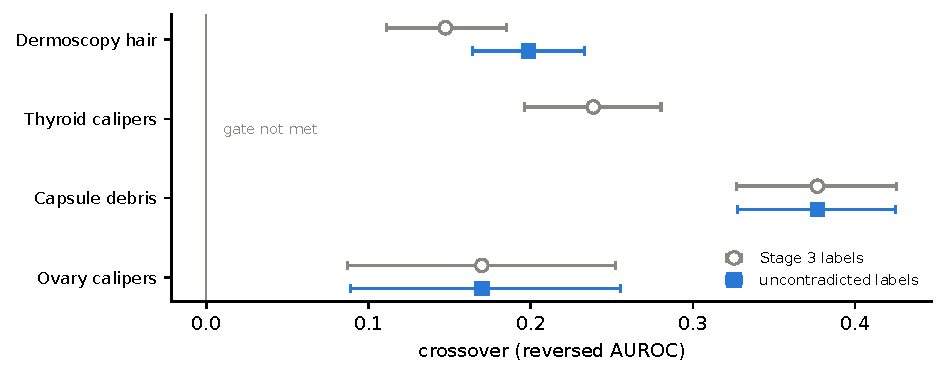
\includegraphics[width=0.8\linewidth]{../stage8_labels_strong_model/figures/cleaned.pdf}
\caption{Crossover on the Stage~3 labels (open circles) and on the images no informative source contradicts (squares),
crossed 95\% CIs. Capsule and ovary: nothing was removed; thyroid: the registered cleaning left too few Trap-B images.}
\label{s8:fig:clean}\end{figure}

\subsubsection{Thyroid calipers: two informative labellers with opposite biases}
BUSClean passes the validity guard (it fires on \sEightBusFreePos{} of our caliper-free images), and both labellers pass
the informativeness rule ($\kappa=$ \sEightBusInf{} and \sEightMgInf). Their presence agreement with our detector is
$\kappa=$ \sEightBusKappa{} (BUSClean) and \sEightMgKappa{} (MedGemma); location agreement is \sEightBusLoc{} on the
\sEightNBusLoc{} images where BUSClean returns positions and \sEightMgLoc{} on \sEightNMgLoc{} images for MedGemma.
Table~\ref{s8:tab:thylab} shows why the registered cleaning failed: the two labellers err in opposite directions. MedGemma
reports a caliper on \sEightMgYestrapA{} of our Trap-A images but also on \sEightMgYesartifactfree{} of our caliper-free
images; BUSClean rarely fires on caliper-free images but finds an annotation on only \sEightBusYestrapA{} of Trap-A images.
Under the registered rule --- remove an image if \emph{any} informative source disagrees --- the two biases add up:
\sEightContratrapA{} of Trap~A and \sEightContratrapB{} of Trap~B are removed, the cleaned Trap~B keeps \sEightGateBYZero{}
benign and \sEightGateBYOne{} malignant caliper images, below the gate of 25, and HA2 cannot be tested for thyroid.
\begin{table}[H]\centering\scriptsize
\caption{Thyroid: how often each independent labeller reports a caliper in each of our cells, and the share of images the registered rule removes (an image is removed if \emph{any} informative labeller places it in another cell).}\label{s8:tab:thylab}
\begin{tabular}{p{3.4cm}p{1.4cm}p{2.8cm}p{2.8cm}p{2.8cm}}\toprule
Our cell & Images & BUSClean: annotation found & MedGemma: caliper ``yes'' & Contradicted (registered rule) \\\midrule
caliper-free & 1{,}801 & 5\% & 29\% & 30\% \\
Trap~A (in the nodule) & 1{,}150 & 56\% & 99\% & 61\% \\
Trap~B (outside) & 326 & 37\% & 87\% & 87\% \\
\bottomrule\end{tabular}
\end{table}

\paragraph{Differential error} The measured location errors are $e_A=$ \sEightBuseA, $e_B=$ \sEightBuseB{} against BUSClean
and $e_A=$ \sEightMgeA, $e_B=$ \sEightMgeB{} against MedGemma. BUSClean's disagreement in Trap~A is smaller for malignant
nodules (\sEightBusDiffA), which is flagged; MedGemma's is not (\sEightMgDiffA{} and \sEightMgDiffB). The cohort is
therefore flagged and no attenuation correction is reported.
\paragraph{Where the two labellers agree (E1, exploratory)} Table~\ref{s8:tab:thycons}. BUSClean and MedGemma give the same
cell for \sEightNBoth{} of \sEightNCells{} images. On these, they agree with our cell for \sEightBothAgree: caliper-free
\sEightConsAgreeartifactfree, Trap~A \sEightConsAgreetrapA, Trap~B \sEightConsAgreetrapB. Counting an image as
contradicted only when both labellers agree against us removes \sEightConsContraartifactfree{} of caliper-free images,
\sEightConsContratrapA{} of Trap~A and \sEightConsContratrapB{} of Trap~B (\sEightConsContraBYZero{} of benign,
\sEightConsContraBYOne{} of malignant). Presence and in-nodule calipers are well supported; the weakest cell is Trap~B,
calipers outside the nodule. The trap re-run under this rule (E1) is prepared and has not been run.
\begin{table}[H]\centering\scriptsize
\caption{Thyroid, \textbf{exploratory}: the images on which BUSClean and MedGemma give the same cell. An image counts as contradicted only if both place it in the same cell and that cell differs from ours.}\label{s8:tab:thycons}
\begin{tabular}{p{3.4cm}p{2.4cm}p{2.0cm}p{2.0cm}p{1.4cm}p{1.4cm}}\toprule
Our cell & Both labellers agree with each other & \ldots\ and with our cell & Contradicted by both & benign & malignant \\\midrule
caliper-free & 1{,}301 & 97\% & 2\% & 2\% & 2\% \\
Trap~A (in the nodule) & 475 & 94\% & 2\% & 3\% & 1\% \\
Trap~B (outside) & 89 & 48\% & 14\% & 11\% & 21\% \\
\bottomrule\end{tabular}
\end{table}

\paragraph{The registered subgroup} Of the \sEightSubN{} malignant test nodules that our detector gives an in-ROI
caliper (FT3), no nodule is contradicted by both labellers, both confirm the caliper inside the nodule for
\sEightSubConfirmed, MedGemma places it inside for \sEightSubMgIn{} and never reports no caliper, and BUSClean finds no
annotation on \sEightSubBusNone. FT3 restricted to the doubly confirmed nodules (E2) is prepared and has not been run.

\subsubsection{Ovary calipers: one usable labeller}
BUSClean fails the validity guard: it fires on \sEightOvBusFreePos{} of our caliper-free ovary images, so on these screens
it detects on-screen annotation and text, not calipers, and is not used. MedGemma is the only labeller left; its presence
agreement with our detector is low, $\kappa=$ \sEightOvMgKappa{} (benign \sEightOvMgKappaYZero, malignant
\sEightOvMgKappaYOne), and at least one of the two is often wrong on these images. Which one is wrong is exactly what the
informativeness rule decides, and with a single model labeller the registered arbiter is the author's blinded rating
(Amendment~2), which has not been done. No ovary image is removed, and the A2 re-run reproduces Stage~3
(Table~\ref{s8:tab:clean}); it is not evidence about the labels.

\subsubsection{Capsule debris: not checkable}
With \sEightNCap{} matched frames the capsule comparison is not feasible by the coverage gate. All \sEightCapEmpty{}
expert masks of these frames mark no contaminated pixel, including the \sEightCapTrapCells{} frames our probe places in a
trap; with so few frames this is not interpreted. As for ovary, the A2 re-run reproduces Stage~3.

\subsubsection{Part B: a fine-tuned thyroid model near the benchmark}
\paragraph{Recipe} Table~\ref{s8:tab:recipe}. ConvNeXt-T (ImageNet-22k), learning rate \sEightLr, \sEightEpochs{} epochs had
the highest validation AUROC (\sEightValAuc; best DINOv2 ViT-B/14 recipe \sEightDinoVal) and was committed before the final
models were trained.
\begin{table}[H]\centering\scriptsize
\caption{Recipe selection on validation images only (B1); no test image was scored. The chosen recipe (bold) was committed before any final model was trained.}\label{s8:tab:recipe}
\begin{tabular}{lccc}\toprule
Architecture & Learning rate & Epochs & Validation AUROC (ERM, seed 42) \\\midrule
ConvNeXt-T (IN-22k) & 3e-5 & 8 & 0.849 \\
ConvNeXt-T (IN-22k) & 3e-5 & 20 & 0.842 \\
ConvNeXt-T (IN-22k) & 1e-4 & 8 & \textbf{0.865} \\
ConvNeXt-T (IN-22k) & 1e-4 & 20 & 0.865 \\
ResNet-50 & 3e-5 & 8 & 0.658 \\
ResNet-50 & 3e-5 & 20 & 0.723 \\
ResNet-50 & 1e-4 & 8 & 0.723 \\
ResNet-50 & 1e-4 & 20 & 0.781 \\
DINOv2 ViT-B/14 & 3e-5 & 8 & 0.838 \\
DINOv2 ViT-B/14 & 3e-5 & 20 & 0.850 \\
DINOv2 ViT-B/14 & 1e-4 & 8 & 0.715 \\
DINOv2 ViT-B/14 & 1e-4 & 20 & 0.804 \\
\bottomrule\end{tabular}
\end{table}

\paragraph{Hypotheses} Table~\ref{s8:tab:ft}. The mean ERM test AUROC is \sEightFTZero, \sEightFTZeroGap{} below the benchmark
of 0.773: by the registered rule the model is \emph{below benchmark}; the frozen probe reached \sEightFrozenAuc. All four tests are
supported after Holm adjustment. On shortcut-conflicting pairs masking lowers the AUROC by \sEightFTOne{} (FT1), while on
all pairs the change is \sEightConallmaskerm{} and on aligned pairs \sEightConeasymaskerm. Group balancing recovers the
conflicting pairs (balanced $-$ mask \sEightConhardbalancedmask), masking and balancing together do not
(\sEightConhardmaskbalancedmask). The trap crossover is \sEightFTFour{} (FT4).
\begin{table}[H]\centering\scriptsize
\caption{Part B: the chosen fine-tuned model on the official patient-disjoint thyroid split (5 seeds $\times$ 4 arms) and in the thyroid traps (10 bootstrap clusters). Crossed bootstrap; Holm over FT1--FT4.}\label{s8:tab:ft}
\begin{tabular}{lp{5.4cm}p{3.0cm}p{1.3cm}p{1.1cm}p{1.9cm}}\toprule
 & Hypothesis & Estimate [95\% CI] & $p$ (one-sided) & Holm $p$ & Verdict \\\midrule
FT0 & ERM test AUROC $\ge0.773$ (descriptive) & 0.769 & --- & --- & below benchmark \\
FT1 & hard-pair AUROC, mask $-$ ERM $<0$ & $-0.102$ [$-0.178, -0.026$] & 0.0040 & 0.0040 & supported \\
FT2 & sensitivity loss (CI $<0$) at $\ge3$ of OP2--OP5 & 4 of 4 & 0.0005 & 0.0015 & supported \\
FT3 & OP2 sensitivity, malignant with in-ROI caliper, mask $-$ ERM $<0$ & $-0.521$ [$-0.642, -0.382$] & 0.0005 & 0.0015 & supported \\
FT4 & thyroid trap crossover $>0$ & $+0.187$ [$+0.111, +0.268$] & 0.0001 & 0.0004 & supported \\
\bottomrule\end{tabular}
\end{table}

\paragraph{Operating points} Table~\ref{s8:tab:opft} and Figure~\ref{s8:fig:op}. Masking lowers sensitivity at every operating
point, at OP2 from \sEightSensErmOPTwo{} to \sEightSensMaskOPTwo{} (\sEightSensOPTwo), and raises specificity (from
\sEightSpecErmOPTwo{} to \sEightSpecMaskOPTwo): thresholds fixed on validation images land at a more conservative point on
the test set once the model is trained on masked images. In the registered subgroup of \sEightSubN{} malignant nodules with
a caliper on the nodule, sensitivity at OP2 falls from \sEightConfErmOPTwo{} to \sEightConfMaskOPTwo{} (\sEightFTThree;
FT3). This test was registered before any result of this model existed.
\begin{table}[H]\centering\scriptsize
\caption{Fine-tuned model, official patient-disjoint thyroid test split: masking at five validation-fixed operating points (crossed bootstrap, thresholds re-estimated in every replicate).}\label{s8:tab:opft}
\resizebox{\linewidth}{!}{\begin{tabular}{lccccc}\toprule
Operating point (fixed on validation) & Sensitivity ERM $\to$ mask & $\Delta$ sensitivity & $\Delta$ specificity & Sensitivity, malignant with in-ROI caliper (ERM $\to$ mask) & $\Delta$ in that subgroup \\\midrule
OP1 max.\ balanced accuracy & 0.781 $\to$ 0.408 & $-0.373$ [$-0.508, -0.243$] & $+0.239$ [$+0.155, +0.345$] & 0.779 $\to$ 0.269 & $-0.510$ [$-0.660, -0.346$] \\
OP2 specificity $\ge0.80$ & 0.747 $\to$ 0.371 & $-0.376$ [$-0.462, -0.297$] & $+0.225$ [$+0.163, +0.291$] & 0.744 $\to$ 0.223 & $-0.521$ [$-0.642, -0.382$] \\
OP3 specificity $\ge0.90$ & 0.542 $\to$ 0.218 & $-0.324$ [$-0.419, -0.228$] & $+0.143$ [$+0.098, +0.198$] & 0.526 $\to$ 0.108 & $-0.418$ [$-0.536, -0.276$] \\
OP4 sensitivity $\ge0.80$ & 0.783 $\to$ 0.423 & $-0.360$ [$-0.439, -0.257$] & $+0.232$ [$+0.159, +0.302$] & 0.779 $\to$ 0.267 & $-0.513$ [$-0.627, -0.371$] \\
OP5 sensitivity $\ge0.90$ & 0.888 $\to$ 0.646 & $-0.242$ [$-0.345, -0.162$] & $+0.240$ [$+0.159, +0.345$] & 0.867 $\to$ 0.510 & $-0.356$ [$-0.497, -0.225$] \\
\bottomrule\end{tabular}}
\end{table}

\begin{figure}[H]\centering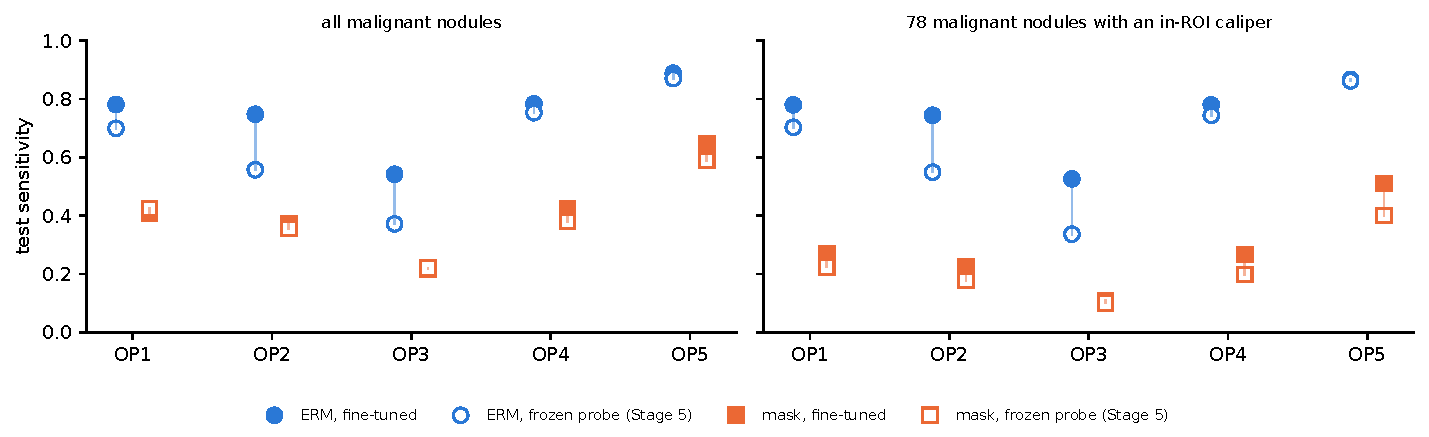
\includegraphics[width=\linewidth]{../stage8_labels_strong_model/figures/op_ft.pdf}
\caption{Test sensitivity of ERM (circles) and of the masked model (squares) at the five validation-fixed operating points,
for the fine-tuned model (filled) and the frozen probe of Stage~5 (open); left: all malignant nodules, right: those with a
caliper on the nodule. Thin lines join the two models.}\label{s8:fig:op}\end{figure}
\paragraph{Against the frozen probe} Table~\ref{s8:tab:cmp}. Every effect is at least as large for the stronger model: the
hard-pair harm (\sEightFrozenHard{} $\to$ \sEightFTOne), the OP2 sensitivity loss, and the subgroup loss
(\sEightFrozenConf{} $\to$ \sEightFTThree). The trap crossover is smaller than the frozen probe's (\sEightFrozenCross) and
larger than that of the fine-tuned ViT-S of Stage~5 (\sEightViTSCross).
\begin{table}[H]\centering\scriptsize
\caption{The same analyses for the frozen probe of Stage~5 and for the fine-tuned model of this stage. The subgroup was post hoc for the probe and registered in advance for the fine-tuned model.}\label{s8:tab:cmp}
\begin{tabular}{p{5.6cm}p{4.2cm}p{4.2cm}}\toprule
Quantity & Frozen DINOv2 ViT-B/14 probe (Stage~5) & Fine-tuned ConvNeXt-T (IN-22k) (this stage) \\\midrule
ERM test AUROC & 0.735 & 0.769 \\
Hard pairs, mask $-$ ERM & $-0.095$ [$-0.165, -0.022$] & $-0.102$ [$-0.178, -0.026$] \\
OP2 sensitivity, mask $-$ ERM & $-0.202$ [$-0.300, -0.100$] & $-0.376$ [$-0.462, -0.297$] \\
OP2 sensitivity, 78 malignant with in-ROI caliper & 0.549 $\to$ 0.177 & 0.744 $\to$ 0.223 \\
\quad change & $-0.372$ [$-0.499, -0.236$] & $-0.521$ [$-0.642, -0.382$] \\
Thyroid trap crossover & $+0.239$ [$+0.196, +0.280$] & $+0.187$ [$+0.111, +0.268$] \\
\bottomrule\end{tabular}
\end{table}


\subsection{What failed or changed}
\begin{itemize}[leftmargin=*]\itemsep1pt
\item \textbf{Hair presence.} The registered hair-free threshold ($\le30$ hair pixels) is far more sensitive than
DermArtifactDB's image-level label ($\kappa=$ \sEightDermKappa), about half of the trap images have no hair by
DermArtifactDB, and the disagreement differs by diagnosis. The hair position is right where hair exists.
\item \textbf{Thyroid HA2 not testable.} The registered ``any source'' rule removed \sEightContratrapB{} of Trap~B, because
the two caliper labellers err in opposite directions; the consensus analysis (E1) is exploratory.
\item \textbf{FT0} is missed by \sEightFTZeroGap{} AUROC: the fine-tuned model is near, not at, the benchmark.
\item \textbf{Capsule} labels could not be checked (\sEightNCap{} frames); \textbf{ovary} labels wait for the rating,
because BUSClean is invalid on ovarian screens. Their ``supported'' HA2 rows reproduce Stage~3 and are not new evidence.
\item \textbf{The rating} (A4, A4b) has not been done; E1 and E2 are prepared and have not been run.
\item \textbf{Reporting corrections after the run} (no estimate changed): the attenuation correction had been printed per
source even where another source of the same cohort flagged differential error, which A3 does not allow; it is now
withheld for both flagged cohorts (dermoscopy, thyroid). For thyroid the withdrawn MedGemma-based value would have been
more than 2.5 times the observed crossover, because $1-e_A-e_B$ is small when a noisy labeller is taken as the truth.
$e_A$ and $e_B$ against DermArtifactDB, which has no location information, had been printed as 0 and are now not defined.
$\kappa$ with the Kabir masks is not informative (our masks mark hair on all \sEightNKabir{} images) and is replaced by the
raw agreement. A committed smoke-test output was removed.
\end{itemize}

\subsection{Anticipated questions}
\paragraph{If DermArtifactDB finds no hair on half of the trap images, are the Stage~3 hair results wrong?} No. Those images
carry weak or no hair, so they dilute the trap; removing every contradicted image makes the crossover larger
(\sEightOrigisic{} $\to$ \sEightCleanisic), and the position of the hair, which is what the law is about, is confirmed
by two independent sources ($e_A+e_B\le$ \sEightImaeSum). The controlled experiments of Stages~2 and~4 place the artifact
themselves and do not use these labels at all.
\paragraph{How can $\kappa$ be so low if the artifact-free cell is almost perfectly clean?} Because the disagreement is
one-sided. Thirty native pixels are a short stretch of a single hair, or a dark line of the lesion, while DermArtifactDB
records whether hair is visible as an artifact. $\kappa$ is dominated by the many images we call hair-bearing and DermArtifactDB
calls hair-free.
\paragraph{Could the differential error have produced the crossover?} It cannot be ruled out from the error rates alone,
which is why the registered rule sends a flagged cohort to A2: without the contradicted images the crossover is larger,
not smaller.
\paragraph{Why did the thyroid cleaning fail if both labellers are informative?} ``Informative'' means $\kappa\ge0.40$, not
unbiased. MedGemma says ``yes'' too often and BUSClean too rarely; a rule that lets either one veto an image removes most
images whenever the two disagree, and they disagree most on calipers outside the nodule.
\paragraph{Is MedGemma a credible labeller?} It is a general medical vision--language model, not a caliper detector, and is
used only through the informativeness rule. Its answers are fixed-prompt, greedy and local, it never sees our masks, and it
is judged against other labels, not trusted: informative for thyroid, undecided for ovary, where its agreement with our
detector is low.
\paragraph{Why is the attenuation correction not reported?} The registration allows it only for cohorts without
differential error, and both cohorts with an informative source are flagged. The correction also treats the source as
the truth; with a noisy labeller it inflates the crossover rather than correcting it.
\paragraph{Is 0.769 ``benchmark-level''?} Not by the registered rule, which is 0.773. The paper can call the model
near-benchmark (\sEightFTZeroGap{} below the lowest published baseline, above the frozen probe) and must not call it
benchmark-level.
\paragraph{Why does sensitivity fall by half while the AUROC barely moves?} The AUROC compares rankings; the operating
points transport a threshold from validation to test. Training on masked images moves the model's test scores relative to
that threshold (specificity rises at every operating point), and the loss is largest in the malignant nodules whose
caliper, the retained shortcut, points to benign.
\paragraph{Why use exploratory analyses at all?} Because the registered rule failed for a structural reason that the
consensus view makes visible. E1 and E2 are reported apart from the registered results and are never tests.

\subsection{Conclusion}
\textbf{Supported.} Where an artifact is present, our labels put it on the correct side of the ROI boundary (dermoscopy,
two independent sources); the dermoscopy crossover survives, and grows, on uncontradicted labels (HA2); a fine-tuned model
near the benchmark shows every registered harm of masking --- on conflicting pairs (FT1), at every operating point (FT2),
in the subgroup of \sEightSubN{} malignant nodules with an in-ROI caliper, registered in advance (FT3), and in the traps (FT4).
\textbf{Qualified.} Hair presence is over-called, with errors that differ by diagnosis; thyroid caliper labels agree with
two independent labellers where those agree with each other, weakest for calipers outside the nodule, but the registered
cleaned-trap test could not run; the fine-tuned model is \sEightFTZeroGap{} below the benchmark. \textbf{Not yet known.}
Whether the ovary caliper labels are right, and the author's blinded rating; the capsule labels cannot be checked with
public data.

\subsection{Questions for the supervisor}
\begin{enumerate}\itemsep1pt
\item Is a clinician-free validation --- public expert annotations, two independent automatic labellers and a blinded
non-clinician rating --- acceptable for the paper, stated as such?
\item Should the paper lead with the cleaned dermoscopy crossover and report the over-called hair presence as a limitation
of the published hair masks at our threshold?
\item May the thyroid clinical result now be stated as registered (FT3), with the model described as near-benchmark?
\item Is the author's rating worth doing now, given that the ovary labels depend on it, or should the ovary real-artifact
evidence be presented as unvalidated?
\end{enumerate}

